\chapter{Implementation and performance}
\label{performance}

This chapter discusses Raft's implementations and its performance for log
replication.

\section{Implementation}

We have implemented Raft as part of LogCabin, a replicated state machine
implemented
as a network service. We initially developed LogCabin to store
configuration information for RAMCloud~\cite{Ousterhout:2011} and assist
in failover of the RAMCloud coordinator. We had planned to implement
Paxos in LogCabin, but the difficulties we faced motivated us to develop
Raft. LogCabin then served as our test platform for new ideas in Raft,
and also as a way to verify that we understood the issues of building a
complete and practical system. The Raft implementation in LogCabin
contains roughly \num{2000} lines of C++ code, not including tests, comments,
or blank lines. The source code is freely available~\cite{logcabin}.
Its architecture is discussed in the next section.

In addition to LogCabin, there are dozens of third-party open-source
implementations of Raft in various stages of
development~\cite{implementations}. Many of these use different
architectures than LogCabin, such as the actor
model~\cite{impl:rafter,impl:akka-raft,impl:archie-raft} or event-based
programming~\cite{impl:kanaka-raft-js,impl:barge,impl:kontiki}. Various
companies are also deploying Raft-based systems~\cite{implementations}.
For example, Facebook is currently testing HydraBase, a fork of Apache
HBase~\cite{HBase}
that uses Raft for replication~\cite{HydraBase}.

\subsection{Threaded architecture}
\label{performance:threads}

\begin{figure}
\centering
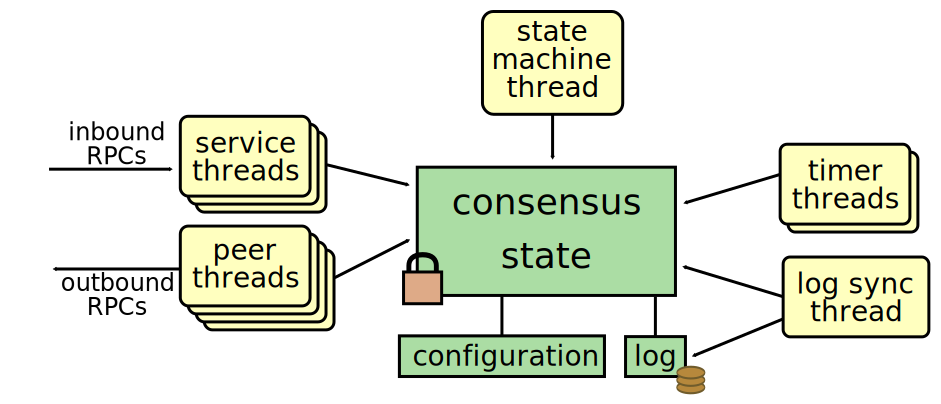
\includegraphics[scale=.4]{performance/threads}
\vcaption[threaded architecture]{
In LogCabin,
consensus state for each server is stored in a monitor protected by a
single lock, accessed by a collection of threads. The threads
communicate with other servers (``peer threads''), handle incoming
requests from clients and other servers (``service threads''), execute
commands in the state machine (``state machine thread''), implement
timeouts (``timer threads''), and write log entries to disk (``log sync
thread'').
}
\label{fig:performance:architecture}
\end{figure}

Raft lends itself to a straightforward implementation architecture using
threads, as shown in Figure~\ref{fig:performance:architecture}. This is
not the only possible architecture, but it is the approach we have taken
in LogCabin. Each server consists of a collection of shared state
variables managed in a monitor style with a single lock.  Five groups of
threads call into the monitor to manipulate the state:
%
\begin{itemize}
%
\item \textbf{Peer threads:} 
%
There are as many peer threads as there are other servers in the
cluster; each peer thread manages the RPCs to one of the other servers.
Each thread enters the consensus state monitor, using a condition
variable to wait for events that require communication with the given
server. Then it leaves the monitor (releasing the lock) and issues an
RPC. Once the RPC completes (or fails), the peer thread reenters the
consensus state monitor, updates state variables based on the RPC, and
waits for the next event that requires communication.
%
\item \textbf{Service threads:}
%
Several threads handle incoming requests from clients and other servers.
These threads wait outside the consensus state monitor for incoming
requests, then enter the monitor to carry out each request.
%
\item \textbf{State machine thread:}
%
One thread executes the state machine. It enters the consensus state
monitor to wait for the next committed log entry; when an entry is
available, it leaves the monitor, executes the command, and returns to
the monitor to wait for the next command.
%
\item \textbf{Timer threads:}
%
One thread manages the election timer for both followers and candidates;
it starts a new election once a randomized election timeout has elapsed.
A second thread causes the server to return to the follower state if, as
leader, it is unable to communicate with a majority of the cluster;
clients are then able to retry their requests with another server (see
Section~\ref{clients:findleader}).
%
\item \textbf{Log sync thread:} When the server is leader, one thread
writes log entries durably to disk. This is done without holding the
lock on the consensus state, so replication to followers can proceed in
parallel; see Section~\ref{performance:leaderdisk}. For simplicity,
followers and candidates write directly to disk from their service
threads while holding the consensus lock; they do not use the log sync
thread.
%
\end{itemize}


\section{Performance considerations}

Raft's performance is similar to other consensus algorithms such as
Multi-Paxos. The most important case for performance is when an
established leader is replicating new log entries. Raft achieves this
using the minimal number of messages (a single round-trip from the
leader to half the cluster). It is also possible to further improve
Raft's performance. For example, Raft easily supports batching and
pipelining requests for higher throughput and lower latency, as
described below. Chapter~\ref{related} discusses various other
optimizations that have been proposed in the literature for other
algorithms; many of these could be applied to Raft, but we leave this to
future work.

Figure~\ref{fig:performance:unoptimizedpipeline} shows the steps Raft
must take to process a client's request. Typically, the most
time-consuming steps are writing the new log entry to disk and
replicating it across the network. Writing to disk can take anywhere
from \SI{100}{\micro\second} for a fast solid state disk to
\SI{10}{\milli\second} for
a slow magnetic disk, while the latencies of today's networks can vary
from \SI{5}{\micro\second} round trip times in highly optimized datacenter
networks to \SI{400}{\milli\second} round trip times for networks that span the
globe. In our experiments on a local area network, either the disk or
the network dominated, depending on which model of solid state disk we
used.

\subsection{Writing to the leader's disk in parallel}
\label{performance:leaderdisk}

\begin{figure}
\centering

\begin{subfigure}{\textwidth}
\centering
\includegraphics[scale=0.50]{performance/unoptimizedpipeline}
\caption{
Unoptimized Raft pipeline.
}
\label{fig:performance:unoptimizedpipeline}
\end{subfigure}

\begin{subfigure}{\textwidth}
\centering
\includegraphics[scale=0.50]{performance/optimizedpipeline}
\caption{
Optimized Raft pipeline.
}
\label{fig:performance:optimizedpipeline}
\end{subfigure}

\vcaption[optimized request processing pipeline]{
To process a client's request in an unoptimized implementation of Raft,
the leader takes the following steps, shown in
\subref{fig:performance:unoptimizedpipeline}: it receives the client's
request, appends it to its local log, flushes the log entry to disk, and
sends out AppendEntries requests. Then, the followers append the entry
to their logs and flush it to their disks. Once the leader receives
positive AppendEntries responses from half of its followers, it marks
the entry committed, applies the entry to its state machine, and replies
to the client. In \subref{fig:performance:optimizedpipeline}, the leader
writes the log entry to its disk in parallel with replicating the entry
to the followers, which can reduce latency significantly.
}
\label{fig:performance:pipeline}
\end{figure}

One useful performance optimization can remove a disk write from Raft's
critical path.
In a na\"ive implementation, the leader writes the new log entry to disk
before replicating the entry to its followers.
Then, the followers write the entry to their disks.
This results in two
sequential disk writes on the path to process a request, contributing
significant latency for deployments where disk writes are a dominant
factor.

Fortunately, the leader can write to its disk in parallel with
replicating to the followers and them writing to their disks; see
Figure~\ref{fig:performance:optimizedpipeline}. To handle this simply,
the leader uses its own \emph{match index} to indicate the latest entry
to have been durably written to its disk. Once an entry in the leader's
current term is covered by a majority of match indexes, the leader can
advance its commit index. The leader may even commit an entry before it
has been written to its own disk, if a majority of followers have
written it to their disks; this is still safe.
LogCabin implements this optimization.

\subsection{Batching and pipelining}

Raft supports batching and pipelining of log entries, and both are
important for best performance. Many of the costs of request processing are
amortized when multiple requests are collected into a batch. For
example, it is much
faster to send two entries over the network in one packet than in two
separate packets, or to write two entries to disk at once. Thus, large
batches optimize throughput and are useful when the system is under
heavy load. Pipelining, on the other hand, optimizes latency under
moderate load by allowing one entry to start to be processed when
another is in progress. For example, while a follower is writing the
previous entry to disk, pipelining allows the leader to replicate the
next entry over the network to that follower. Even at high load, some
amount of pipelining can increase throughput by utilizing resources more
efficiently. For example, a follower needs to receive entries over the
network before it can write them to disk; no amount of batching can use
both of these resources at once, but pipelining can. Pipelining also
works against batching to some degree. For example, it might be faster
overall to delay requests and send one big batch to followers, rather
than pipelining multiple small requests.

Batching is very natural to implement in Raft, since AppendEntries
supports sending multiple consecutive entries in one RPC. Leaders in
LogCabin send as many entries as are available between the follower's
\emph{next index} and the end of the log, up to one megabyte in size. The one
megabyte limit is arbitrary, but it is enough to use the network and
disk efficiently while still providing frequent heartbeats to followers
(if one RPC got to be too large, the follower might suspect the leader
of failure and start an election). The follower then writes all the new
entries from a single AppendEntries request to its disk at once, thus
making efficient use of its disk.

Pipelining is also well-supported by Raft. The AppendEntries consistency
check guarantees that pipelining is safe; in fact, the leader can safely
send entries in \emph{any} order. To support pipelining, the leader
treats the next index for each follower optimistically; it updates the next index
to send immediately after sending the previous entry, rather than
waiting for the previous entry's acknowledgment. This allows another
RPC to pipeline the next entry behind the previous one. Bookkeeping is a
bit more involved if RPCs fail. If an RPC times out, the leader must
decrement its next index back to its original value to retry. If the
AppendEntries consistency check fails, the leader may decrement the next
index even further to retry sending the prior entry, or it may wait for
that prior entry to be acknowledged and then try again. Even with this
change, LogCabin's original threading architecture still prevented
pipelining because it could only support one RPC per follower; thus, we
changed it to spawn multiple threads per peer instead of just one.
%

This approach to pipelining works best if messages are expected to be
delivered in order in the common case, since reordering may lead to
inefficient retransmissions. Fortunately, most environments will not
reorder messages often. For example, a leader in LogCabin uses a single
TCP connection to each follower, and it only switches to a new
connection if it suspects a failure. Since a single TCP connection masks
network-level reordering from the application, it is rare for LogCabin
followers to receive AppendEntries requests out of order. If the network
were to commonly reorder requests, the application could benefit from
buffering out-of-order requests temporarily until they could be appended
to the log in order.

The overall performance of a Raft system depends greatly on how batches
and pipelines are scheduled. If not enough requests are accumulated in
one batch under high load, overall processing will be inefficient,
leading to low throughput and high latency. On the other hand, if too
many requests are accumulated in one batch, latency will be needlessly
high, as early requests wait for later requests to arrive.


While we are still investigating the best policy, our goal is to
minimize the average delay for requests under dynamic workloads. Before
we had implemented pipelining in LogCabin, it used a simple
double-buffering technique. The leader would keep one outstanding RPC to
each follower. When that RPC returned, it would send another one with
any log entries that had accumulated in the meantime, and if no more
entries were available, the next RPC would be sent out as soon as the
next entry was appended. This approach is appealing because it
dynamically adjusts to load. As soon as load increases, entries will
accumulate, and the next batch will be larger, improving efficiency.
Once load decreases, batches will shrink in size, lowering latency. We
would like to retain this behavior for pipelining. Intuitively, in a
two-level pipeline, we would like the second batch to be started halfway
through the processing time for the first batch, thus halving the
average delay. However, guessing when a batch is halfway done requires
estimating the round-trip time; we are still investigating the best
policy to use in LogCabin.


\section{Preliminary performance results}

\begin{table}
\centering
\begin{tabular}{r l}
code & LogCabin~\cite{logcabin}, written in C++11 \\
OS & x86-64 RHEL6 (Linux 2.6.32) \\
CPU & Xeon X3470 (4 cores, 8 hyperthreads) \\
disk & ext4 file system on Intel DC S3500 SSDs (1 SSD per server; write
caching off) \\
network & Protocol Buffers~\cite{Varda:2008} over TCP/IP over 1~gigabit Ethernet \\
configuration & in-memory state machine, no log compaction
\end{tabular}
\vcaption[experimental setup]{
Experimental setup.
}
\label{tab:performance:setup}
\end{table}

We have not yet analyzed the performance of LogCabin in depth, but we
have taken some initial measurements. The experimental setup is
summarized in Table~\ref{tab:performance:setup}. In the benchmark, a
single client process connects to the leader of a LogCabin cluster.
Varying numbers of client threads issue operations to the replicated state machine
to set a \SI{1024}{byte} value. Each client thread repeatedly issues a
request on a shared TCP connection, waits for the result from the
leader's state machine, then issues its next request.

\begin{figure}
\centering
\captionsetup[subfigure]{singlelinecheck=false,
                         margin={2em}}

\begin{subfigure}{\textwidth}
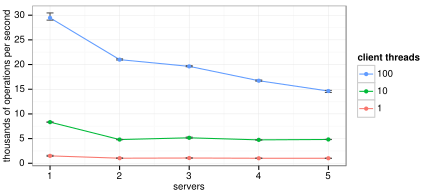
\includegraphics[scale=1]{performance/throughput}
\caption{
Throughput.
}
\label{fig:performance:throughput}
\end{subfigure}

\vspace{3ex}

\begin{subfigure}{\textwidth}
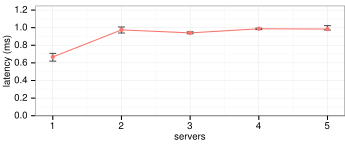
\includegraphics[scale=1]{performance/latency}
\caption{
Latency.
}
\label{fig:performance:latency}
\end{subfigure}

\vcaption[preliminary measurements of LogCabin]{
Preliminary latency and throughput measurements of LogCabin. In
each test, a single client process connects to the leader of a LogCabin
cluster of varying size. In \subref{fig:performance:throughput}, varying
numbers of client threads issue operations to the state machine to set a
\SI{1024}{byte} value; in \subref{fig:performance:latency}, only one
client thread is used. Each client thread repeatedly issues a request on
a shared TCP connection, waits for the result from the leader's state
machine, then issues its next request. Each data point represents the
mean of five runs of approximately \SI{10}{seconds} each; error bars
show the minimum and maximum values across the five runs (the range is
very small for most points).
}
\end{figure}

Figure~\ref{fig:performance:throughput} shows the current throughput of
LogCabin. Using a multi-threaded client with 100 threads, a three-server
cluster sustains about \num{19500} kilobyte-sized writes per second.
As expected, performance degrades when using larger clusters, since the
leader has to send each entry to a larger number of followers.


Figure~\ref{fig:performance:latency} shows the current latency of
LogCabin. The latency for a kilobyte-sized write is about
\SI{0.7}{\milli\second} for a single-server cluster and
about \SI{1.0}{\milli\second} for two- to five-server clusters.
This includes the time to write one kilobyte durably to disk,
which we measured in a microbenchmark to be about \SI{.25}{\milli\second}.

The initial measurements are encouraging, and we think the current
performance would be sufficient for a large class of applications.
However, there is still much room for improvement. For example, gigabit
Ethernet would limit the performance of a three-server cluster to
about \num{60000} kilobyte-sized writes per second, and
LogCabin's current throughput is only one third of that.


\section{Conclusion}

There are many performance aspects of Raft we would like to analyze in
the future. Most importantly to normal operation, we would like to
analyze the latency and throughput for write operations and for
read-only operations under varying load. There are various performance
questions that arise during exceptional circumstances that we would also
like to analyze:
%
\begin{compactitem}
%
\item How quickly do clients find the leader?
%
\item How quickly does a new leader commit its first entry, including
how quickly does a leader discover where its followers' logs diverge?
%
\item What is the effect of follower failures on normal operation?
%
\item How long does it take to reconfigure the cluster, and what is its
effect on normal operation?
%
\item How long does it take to compact the log, and what is its effect
on normal operation?
%
\item How long does it take a server/cluster to restart?
%
\end{compactitem}

Our performance goal with Raft was to match current algorithms such as
Multi-Paxos, while improving understandability. Rather than wanting to
build the fastest system, we wanted to enable others to build
consensus-based systems that were competitive in performance.
Though LogCabin is not yet well-optimized, preliminary results show
that it achieves reasonable latency and throughput: writing
kilobyte-sized objects to a three-server cluster takes about
\SI{1.0}{\milli\second} per operation with a single client thread, and the
system processes \num{19500} operations per second when using 100 client
threads.
